\subsection{Bestimmung der Stoffmenge} \label{sec:Stoffmenge}
In Aufgabe drei sollte die Berechnung Stoffmenge über eine Interpolation zu einem Volumen erfolgen. Hierzu wird ein $\frac{1}{V}$ -- $pV$--Diagramm erstellt und der y-Achsenabschnitt über ein Ausgleichspolynom 3ter Ordnung ermittelt (Reihenentwicklung, siehe Abbildung \ref{fig:aufgabe3}).\footnote{Berechnung durch Origin} Bei der Interpolation ergibt sich für $y$ bei $x=0$ der Wert $y=\unit[(7.56 \pm 0.39)]{J}  $. Aus der Gleichung für ideale Gase, ergibt sich für den Druck $p [\mathrm{100kPa}]$, das Volumen $V [\mathrm{cm^3}]$, die Stoffmenge $n_2 [\mathrm{mmol}]$ (Für die Temperatur von Gruppe zwei von $\unit[50]{^\circ C} > T_{krit}$), die allgemeine Gaskonstante $R [\mathrm{\frac{J}{mol \cdot K}}]$ und die Temperatur $T [\mathrm{K}]$:

\begin{align}
p \cdot V &= n_2 \cdot R \cdot T\\
n_2 &= \frac{p \cdot V}{R \cdot T} \approx \unit[(22.86 \pm 0.02)]{mmol} \notag
\end{align}
Der Fehler ergibt sich durch:
\[
F = \sqrt{F_{stat}^2 + F_{sys}^2}
\]
Wobei $F_{stat} = \unit[0.01]{mmol}$. Der systematische Fehler des Thermometers liegt bei $\unit[0.2]{^\circ C}$, somit ergibt sich ein systematischer Fehler für $n$ von $F_{sys} = \unit[0.017]{mmol}$, der Gesamtfehler ergibt sich demnach zu $F = \unit[0.022]{mmol}$. \\
Für die später benötigten Stoffmengen $n_1$ ($\unit[47.5]{^\circ C}$) und $n_3$ ($\unit[55]{^\circ C}$) ergeben sich folgende Werte.
\begin{align*}
n_1 &= \unit[(22.86 \pm 0.02)]{mmol}\\
n_3 &= \unit[(20.36 \pm 0.02)]{mmol}
\end{align*}

\begin{figure}
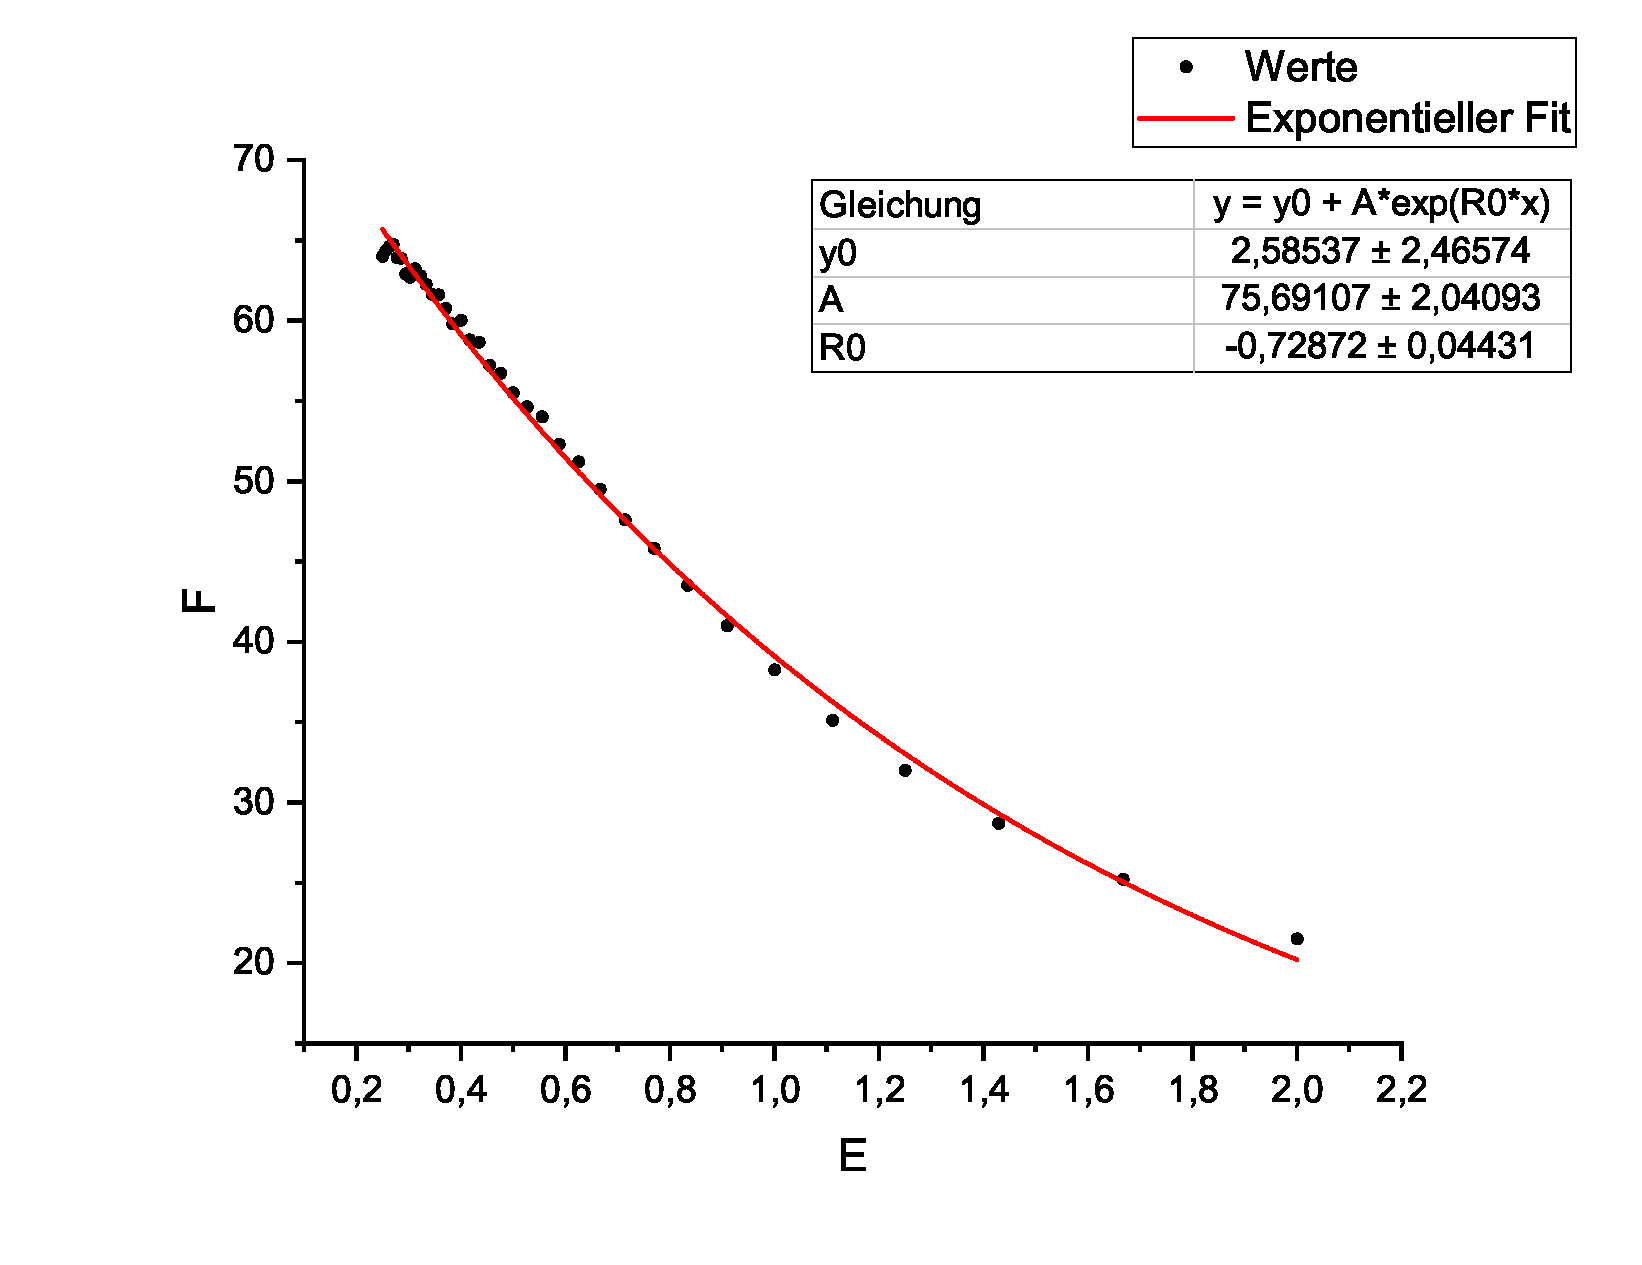
\includegraphics[width=0.9\textwidth]{Bilder/aufgabe_3.eps}
\caption{Ermittlung der Stoffmenge $n_2$}
\label{fig:aufgabe3}
\end{figure}